\chapter{Classical string motion on a general background}
\label{chap:general_background}

In this chapter, we will develop some fundamental tools for acquiring the equations of motion of a~classical relativistic string. Let us first summarize the motion of a~single classical relativistic particle, which is described in detail in \cite{zwiebach}.

%%%%%%%%%%%%%%%%%%%%%%%%%%%%%%%%%% SECTION %%%%%%%%%%%%%%%%%%%%%%%%%%%%%%%%%%%%%%%%%%%%%%

\section{Motion of classical relativistic particle}

In classical relativistic mechanics a~particle moves along a~curve in spacetime called a~world-line. This curve can be parametrized in many ways, but the physics have to be invariant of the choice of parameterization. When we want to find this world-line, we usually use the action principle. The action of a~world-line is proportional to its Lorentz invariant ``proper length", which in turn is equal to the proper time associated with this world-line times the factor $c = 1$. The infinitesimal proper time $\D \lambda$ for a~particle with mass takes the form

\begin{equation}
    -\D \lambda^2 = \D s^2 = g_{M N}(X) \D X^{M} \D X^{N} 
\end{equation}

\noindent
where $g_{MN}$ is the metric of the spacetime.

Since the proper time has the units of time, we need an additional multiplicative factor to get the units of action, which is energy $\times$ time. The energy of a~static particle would be $E = m c^2$, but we put $c = 1$, therefore the multiplicative factor will be $m$. Also, since the proper time is always positive, we will add a~$ - $~sign so that the extrema of the action is a~minimum. This does not change anything from the mathematical point of view, but it is a~convention in physics. The action of such a~particle is then

\begin{equation}
    S = -m \int \D \lambda = - \int {\sqrt{-\D s^2}}
\end{equation}

\noindent
If we choose a~specific parameter $\tau$

\begin{equation*}
X^{M} = X^{M}(\tau),
\end{equation*}

\noindent
we can express the action in the following form

\begin{equation}
    S = -m \int\limits_{\tau_i}^{\tau_f} \sqrt{-g_{MN}(X) \dif[] {X^{M}} {\tau} \dif[]{X^{N}}{\tau}} \D \tau
\end{equation}

\noindent
From the variation of this action, we acquire the geodesic equation (equations of motion) for a~particle in a~space with metric $g_{MN}$.

%%%%%%%%%%%%%%%%%%%%%%%%%%% SECTION %%%%%%%%%%%%%%%%%%%%%%%%%%%%%

\section{String action}
\label{sec:string_action}

Let us now turn towards the classical relativistic strings and find the action associated with them. Just as a~particle traces out a~curve in spacetime called a~world-line, a~string traces out a~two dimensional surface called a~world-sheet. There can be two types of strings. A~closed string that traces out a~tube and an open string that traces out a~strip as seen in \cref{fig:particle_vs_string}. 

\begin{figure}
\centering

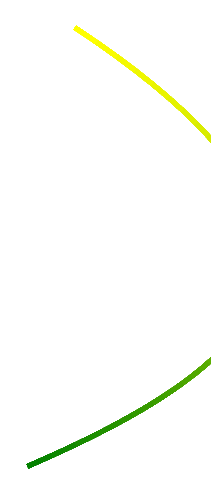
\begin{tikzpicture}
  \begin{axis}[
    hide axis,
    view = {20}{20},
    xscale = 0.6,
    yscale = 1.2
  ]
    \addplot3[variable=t,
    mesh,
    colormap/greenyellow,
    samples = 50,
    ultra thick,
    domain=0:1] ({exp(t)*cos(70*t)}, {exp(t)*sin(70*t)}, t);
  \end{axis}
\end{tikzpicture}
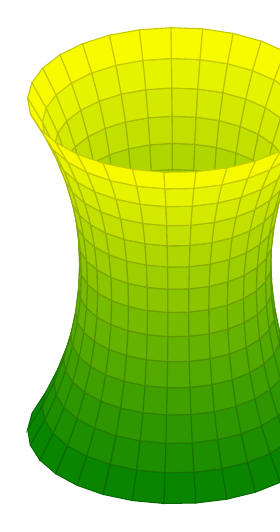
\begin{tikzpicture}
  \begin{axis}[
    hide axis,
    view = {20}{20},
    xscale = 0.7,
    yscale = 1.3
  ]
  \addplot3 [
    surf,
    colormap/greenyellow, 
    %shader     = flat,
    point meta = z,
    samples    = 30,
    samples y  = 15,
    z buffer   = sort,
    domain     = 0:360,
    y domain   =-4:4
  ] (
    {cosh(y/4)*cos(x)},
    {cosh(y/4)*sin(x)},
    {y}
  );
  \end{axis}
\end{tikzpicture}
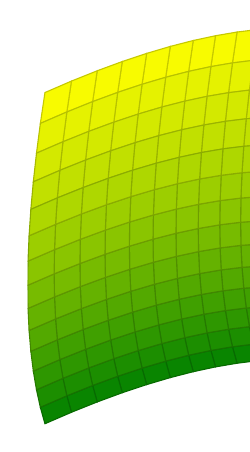
\begin{tikzpicture}
  \begin{axis}[
    hide axis,
    view = {20}{20},
    xscale = 0.6,
    yscale = 1.3
  ]
  \addplot3 [
    surf,
    colormap/greenyellow,
    %shader     = faceted interp,
    point meta = z,
    samples    = 15,
    samples y  = 15,
    z buffer   = sort,
    domain     = 0:2,
    y domain   =-1:1
  ] (
    {-x},
    {-(x^2-y^2)/2},
    {y}
  );
  \end{axis}
\end{tikzpicture}

\caption{Trajectory of a~particle (left) vs a~closed string (middle) vs an~open string (right).}
\label{fig:particle_vs_string}

\end{figure}

In the previous section, we found that the action of a~particle is proportional to its Lorentz invariant ``proper length". In a~similar way, we will define a~Lorentz invariant ``proper area" of a~world-sheet. The action of a~classical relativistic string, called the Nambu--Goto action, is proportional to this two dimensional proper area $\D A$.

\begin{equation}
    S = -T_0 \int \D A
\end{equation}

\noindent
where $T_0$ is again a~multiplicative factor to get the units of action and has the meaning of tension of the string and its units are energy / length. The infinitesimal area $\D A$ has units of length $\times$ time, so the units of the action are, again, energy $\times$ time.

In order to parameterize the world-sheet, we require two parameters $\xi^1$ and $\xi^2$. The surface is described by the collection of functions 

\begin{equation}
    X^M = X^M (\xi^1, \xi^2)
\end{equation}

\noindent
Also, we will call the \textit{target space} the space where the strings propagate. We can define an induced metric on the world-sheet as

\begin{equation}
\label{eq:gamma_def}
    \gamma_{\alpha \beta} = g_{MN} \dif[]{X^M}{\xi^\alpha} \dif[]{X^N}{\xi^\beta} = g_{MN} ~ \difs[]{X^M}{\alpha} ~ \difs[]{X^N}{\beta}
\end{equation}

\noindent
The area element $\D A$ can be defined as a~square root of the metric. Since we want this element to be expressed in terms of the tangent vectors to the world-sheet $\pardif[]{ }{\xi^1}$ and $\pardif[]{ }{\xi^2}$, we will use the induced metric.

\begin{equation}
    \D A = \sqrt{- \det{\gamma}} \D \xi^1 \D \xi^2
\end{equation}

\noindent
where the $-$ sign corresponds to the fact, that the determinant of the induced metric is always negative. Furthermore, we will name the parameters $\xi^1 = \tau$ and $\xi^2 = \sigma$ and denote $\det \gamma$ as $\gamma$ written without indices. The Nambu--Goto action of a~classical string is then given by

\begin{equation}
\label{eq:action}
    \begin{aligned}
        S &= -T_0 \int\limits_{\tau_i}^{\tau_f} \D \tau \int\limits_{0}^{\sigma_1} \D \sigma ~ \sqrt{- \gamma} =
        - T_0\int\limits_{\tau_i}^{\tau_f} \D \tau \int\limits_{0}^{\sigma_1} \D \sigma ~ \sqrt{\gamma_{\tau \sigma} \gamma_{\sigma \tau} - \gamma_{\tau \tau} \gamma_{\sigma \sigma} } \\
        &= - T_0\int\limits_{\tau_i}^{\tau_f} \D \tau \int\limits_{0}^{\sigma_1} \D \sigma ~ \sqrt{ \lp g_{MN} \difs[]{X^M}{\tau} \difs[]{X^N}{\sigma} \rp ^2 - \lp g_{MN} \difs[]{X^M}{\tau} \difs[]{X^N}{\tau} \rp \lp g_{KL} \difs[]{X^K}{\sigma} \difs[]{X^L}{\sigma} \rp  }
    \end{aligned}
\end{equation}


%%%%%%%%%%%%%%%%%%%%%%%%%%% SECTION %%%%%%%%%%%%%%%%%%%%%%%%%%%%%%%%%

\section{Equations of motion}
\label{sec:general_EOM}

To get the equations of motion, we have to find the minima of the action. At the minima, the first variation of the action has to be zero. We could immediately insert a~metric and choose a~coordinate system in which we would get the equations of motion after the variation. 
%We will not do this here, but we will show an example in later sections, i.e. \cref{sec:check_lagrangian_flat}. 
We will not do that, instead, we will further develop the $\gamma$ notation and obtain a~more convenient general form of the equations of motion. The variation of this action takes the form

\begin{equation}
    \delta S = -T_0 \int\limits_{\tau_i}^{\tau_f} \D \tau \int\limits_{0}^{\sigma_1} \D \sigma ~ \delta \sqrt{- \gamma} = -T_0 \int\limits_{\tau_i}^{\tau_f} \D \tau \int\limits_{0}^{\sigma_1} \D \sigma ~ \frac{-\delta \gamma}{ 2 \sqrt{ - \gamma}}
\end{equation}

\noindent
The variation of the~determinant is given by

\begin{equation}
\begin{aligned}
    \delta (\det \gamma) & = 
    \delta \lp \frac{1}{n!} \varepsilon^{\alpha_1 \dots \alpha_n} \varepsilon^{\beta_1 \dots \beta_n} 
    \gamma_{\alpha_1 \beta_1} \dots \gamma_{\alpha_n \beta_n} \rp \\
    & = \lp \frac{1}{(n-1)!} \varepsilon^{\alpha_1 \dots \alpha_n} \varepsilon^{\beta_1 \dots \beta_n}
    \gamma_{\alpha_1 \beta_1} \dots \gamma_{\alpha_{i-1} \beta_{i-1}} \gamma_{\alpha_{i+1} b_{i+1}} \dots \gamma_{\alpha_n \beta_n} \rp \delta \gamma_{\alpha_i \beta_i} \\
    & = \det (\gamma) \gamma^{\alpha \beta} \delta \gamma_{\alpha \beta}
\end{aligned}
\end{equation}

\noindent
We can now rewrite the variation of the action as

\begin{equation}
\label{eq:var_action1}
    \delta S =  T_0 \int\limits_{\tau_i}^{\tau_f} \D \tau \int\limits_{0}^{\sigma_1} \D \sigma ~ \frac{1}{2} \sqrt{-\gamma}~ \gamma^{\alpha \beta} ~ \delta \gamma_{\alpha \beta}
\end{equation}

\noindent
Using \cref{eq:gamma_def} and the fact that the metric components $g_{M N}$ depend only on $X^K$, the variation of the induced metric $\gamma_{\alpha \beta}$ takes the form

\begin{equation}
\label{eq:var_gamma1}
    \begin{aligned}
        \delta \gamma_{\alpha \beta} = \delta \lp g_{M N}~ \difs[] {X^{M}} {\alpha} ~ \difs[] {X^{N}} {\beta} \rp = \pardif[] {g_{M N}} {X^{K}} \delta X^{K} ~ \difs[] {X^{M}} {\alpha} \difs[] {X^{N}} {\beta} \\
        + g_{M N} ~ \delta \lp \difs[] {X^{M}} {\alpha}\rp \difs[] {X^{N}} {\beta} + g_{M N} ~ \difs[] {X^{M}} {\alpha} ~ \delta \lp \difs[] {X^{N}} {\beta} \rp
    \end{aligned}
\end{equation}

\noindent
Because of the symmetry of both metrics $g_{M N} = g_{N M}$, $\gamma_{\alpha \beta} = \gamma_{\beta \alpha}$ we can show that the second and third term in \cref{eq:var_gamma1} is the same.

\begin{equation}
    \begin{aligned}
        \gamma^{\alpha \beta} g_{M N} ~ \delta \lp \difs[] {X^{M}} {\alpha}\rp \difs[] {X^{N}} {\beta} = 
        \begin{vmatrix}{\alpha \leftrightarrow \beta} \\ {M \leftrightarrow N} \end{vmatrix}
        & = \gamma^{\beta \alpha} g_{N M} ~ \delta \lp \difs[] {X^{N}} {\beta}\rp \difs[] {X^{M}} {\alpha}  \\
        & = \gamma^{\alpha \beta} g_{M N} ~ \difs[] {X^{M}} {\alpha} ~ \delta \lp \difs[] {X^{N}} {\beta}\rp 
    \end{aligned}
\end{equation}

\noindent
Substituting \cref{eq:var_gamma1} into \cref{eq:var_action1} yields:

\begin{equation}
\label{eq:gen_s_before_perpartes}
    \begin{aligned}
        \delta S = - \frac{T_0}{2} \int\limits_{\tau_i}^{\tau_f} \D \tau \int\limits_{0}^{\sigma_1} \D \sigma ~
        \sqrt{-\gamma} ~\gamma^{\alpha \beta} \lp \pardif[] {g_{M N}} {X^{K}} ~ \difs[] {X^{M}} {\alpha} \difs[] {X^{N}} {\beta} ~ \delta X^{K} + 2 ~ g_{M N} ~ \difs[] {X^{M}} {\alpha} \difs[] {\delta X^{N}} {\beta} \rp
    \end{aligned}
\end{equation}

\noindent
If we want to factor out $\delta X^{K}$, we need to integrate by parts the second term in \cref{eq:gen_s_before_perpartes}


\begin{equation}
\label{eq:per_partes}
    \begin{aligned}
     - T_0 \int\limits_{\tau_i}^{\tau_f} \D \tau \int\limits_{0}^{\sigma_1} \D \sigma ~ \sqrt{-\gamma} ~ \gamma^{\alpha \beta} g_{M N} ~ \difs[] {X^{M}} {\alpha} \difs[] {\lp \delta X^{N}\rp} {\beta} \\
     = - T_0 \int\limits_{\tau_i}^{\tau_f} \D \tau \int\limits_{0}^{\sigma_1} \D \sigma ~ \left[
     \difs[] {\lp \sqrt{-\gamma} ~ \gamma^{\alpha \beta} g_{M N} ~ \difs[] {X^{M}} {\alpha} ~ \delta X^{N} \rp} {\beta} \right. \\
     \left. - \difs[] {\lp \sqrt{-\gamma} ~ \gamma^{\alpha \alpha} g_{M N} ~ \difs[] {X^{M}} {\beta} \rp} {\beta}  ~ \delta X^{N}
     \right] 
     \end{aligned}
\end{equation}

\noindent
The first term is a~total derivative. This implies, that it needs to vanish at the boundary. For now, we will assume, that they do, but we will touch on this topic in more detail in \cref{sec:boundary_conditions}. 

We will now focus our attention on the remaining terms and we arrive at a~convenient form of the variation of action:

\begin{equation}
\label{eq:final_gen_action}
\begin{aligned}
    \delta S = - \frac{T_0}{2} \int\limits_{\tau_i}^{\tau_f} \D \tau \int\limits_{0}^{\sigma_1} 
    \D \sigma  \left[ \sqrt{-\gamma} ~ \gamma^{\alpha \beta} ~
    \difs[] {g_{M N}} {K} ~ \difs[] {X^{M}} {\alpha} ~ \difs[] {X^{N}} {\beta} \right. \\
    \left. -2 \difs[] {\lp \sqrt{-\gamma} ~ \gamma^{\alpha \beta} g_{K N} ~ \difs[] {X^{N}} {\beta} \rp} {\alpha} \right] \delta X^{K}
\end{aligned}
\end{equation}

\noindent
This first variation of the action must be zero for any $\delta X^{K}$ for a minimal trajectory. This implies, that the term on the inside of the square brackets in \cref{eq:final_gen_action} must be zero:

\begin{equation}
\label{eq:EL}
        2 ~ \difs[] {\lp \sqrt{-\gamma} ~ \gamma^{\alpha \beta} g_{K N} ~ \difs[] {X^{N}} {\beta} \rp} {\alpha}  - \sqrt{-\gamma} ~\gamma^{\alpha \beta} ~ \pardif[] {g_{M N}} {X^{K}} ~ \difs[] {X^{M}} {\alpha} ~ \difs[] {X^{N}} {\beta} = 0
\end{equation}

\noindent
Together with the boundary conditions, these equations, that are the equivalent of the Euler--Lagrange equations from classical mechanics, fully specify the motion of a~classical relativistic string.


%%%%%%%%%%%%%%%%%%%%%%%%%%%%% BOUNDARY CONDITIONS %%%%%%%%%%%%%%%%%%%%%%%%%%%%%


\section{Boundary conditions}
\label{sec:boundary_conditions}


In this section, we will be interested in terms, that must vanish at the boundary. Specifically, it is the first term in \cref{eq:per_partes} that has to vanish

\begin{equation}
    - T_0 \int\limits_{\tau_i}^{\tau_f} \D \tau \int\limits_{0}^{\sigma_1} \D \sigma ~ 
     \difs[] {\lp \sqrt{-\gamma} ~ \gamma^{\alpha \beta} g_{M N} ~ \difs[] {X^{M}} {\alpha} ~ \delta X^{N} \rp} {\beta} = 0
\end{equation}

\noindent
To better understand what this equation means, we will use Stokes' theorem. If we denote 

\begin{equation}
\label{eq:form_ppts}
    \omega = \sqrt{-\gamma} ~ \gamma^{\alpha \beta} g_{M N} ~ \difs[] {X^{M}} {\alpha} ~ \delta X^{N}
\end{equation}

\noindent
We can take an outer derivative 

\begin{equation}
\label{eq:diff_form_ppts}
    \D \omega = \difs[] {\lp \sqrt{-\gamma} ~ \gamma^{\alpha \beta} g_{M N} ~ \difs[] {X^{M}} {\alpha} ~ \delta X^{N} \rp} {\beta} \D y^{\beta}
\end{equation}

\noindent
where $\D y^{\beta}$ is a coordinate basis vector in the tangent space of the manifold over which we integrate. This manifold corresponds to our world-sheet. Using the Stokes' theorem

\begin{equation}
\label{eq:stokes}
    \int\limits_{V} \D \omega = \int\limits_{\partial V} \omega
\end{equation}

\noindent
we conclude, that if we have an integral over some part of a manifold, like the one in \cref{eq:per_partes}, we can transform it to an integral over the boundary of this manifold. We can always choose $\tau$ and $\sigma$ to be perpendicular. When this is true, we can split the integral over the boundary into four integrals.

\begin{equation}
\label{eq:boundary_integrals}
    \begin{aligned}
    \int\limits_{\partial V} \omega  & = 
    \int\limits_{\tau_i}^{\tau_f} \D \tau ~ \left[ \sqrt{-\gamma} ~ \gamma^{\alpha \sigma} g_{M N} ~ \difs[] {X^{M}} {\alpha} ~ \delta X^{N} \right]_{\sigma = 0} \\
    & + \int\limits_{0}^{\sigma_1} \D \sigma ~ \left[ \sqrt{-\gamma} ~ \gamma^{\alpha \tau} g_{M N} ~ \difs[] {X^{M}} {\alpha} ~ \delta X^{N} \right]_{\tau = \tau_f} \\
    & +\int\limits_{\tau_f}^{\tau_i} \D \tau ~ \left[ \sqrt{-\gamma} ~ \gamma^{\alpha \sigma} g_{M N} ~ \difs[] {X^{M}} {\alpha} ~ \delta X^{N} \right]_{\sigma = \sigma_1} \\
    & + \int\limits_{\sigma_1}^{0} \D \sigma ~ \left[ \sqrt{-\gamma} ~ \gamma^{\alpha \tau} g_{M N} ~ \difs[] {X^{M}} {\alpha} ~ \delta X^{N} \right]_{\tau = \tau_i}
    \end{aligned}
\end{equation}

\noindent
For easier manipulation, we will denote part of the inside of these integrals as

\begin{align}
\label{eq:denote_p}
    \mathcal{P}^{\tau}_{N} & = \pardif{\mathcal{L}}{(\difs[]{X^N}{\tau})} = T_0 \sqrt{-\gamma} ~ \gamma^{\alpha \tau} g_{M N} ~ \difs[] {X^{M}} {\alpha} \\[10pt]
    \mathcal{P}^{\sigma}_{N} & = \pardif{\mathcal{L}}{(\difs[]{X^N}{\sigma})} = T_0 \sqrt{-\gamma} ~ \gamma^{\alpha \sigma} g_{M N} ~ \difs[] {X^{M}} {\alpha}
\end{align}

\noindent
Also, we will restrict ourselves to variations with fixed endpoints in proper time, such that $\delta X^M (\tau_i, \sigma) = \delta X^M (\tau_f, \sigma) = 0$. In that case, the second and fourth term do not contribute. Therefore, the boundary conditions impose

\begin{equation}
\label{eq:boundary_integrals_compact}
    T_0 \int\limits_{\partial V} \omega = - \int\limits_{\tau_i}^{\tau_f} \D \tau ~ \left[ \mathcal{P}^{\tau}_{N} ~ \delta X^{N} \right]_{0}^{\sigma_1} = 0
\end{equation}

\noindent
These terms must vanish at every boundary $\sigma_b \in \{0, \sigma_1 \}$. This can be ensured when either $\mathcal{P}^{\tau}_{N}$ or $\delta X^{N}$ are zero at the boundary. The former case is called the free endpoint boundary condition, because it does not impose any restriction to $\delta X^N(\tau, \sigma_b)$. The later case is called the Dirichlet boundary condition. This means, that the string endpoint is fixed throughout the motion. This can also be expressed as $\difs[]{X^N}{\tau}(\tau, \sigma_b)$ being equal to zero.

\begin{align}
\label{eq:dirichlet_boundary}
    \text{Dirichlet boundary condition:} & \qquad \difs[] {X^{N}} {\tau} (\tau, \sigma_b) = 0\\[15pt]
    \text{free endpoint boundary condition:} & \qquad \mathcal{P}^{\tau}_{N} (\tau, \sigma_b) = 0
\end{align}
\vspace{0mm}

\noindent

\noindent
Open strings have to satisfy at least one condition for every component $N$. We must be careful with the choice of boundary conditions. For example, we cannot choose a~Dirichlet boundary condition for the~time-like coordinate component, because the time-like coordinate has to change with proper time. 

For closed strings, the terms in \cref{eq:boundary_integrals_compact} always cancel out, because $X^N(\tau, 0) = X^N (\tau, \sigma_1)$.